\documentclass[11pt,]{article}
\usepackage[left=1in,top=1in,right=1in,bottom=1in]{geometry}
\newcommand*{\authorfont}{\fontfamily{phv}\selectfont}
\usepackage[]{mathpazo}


  \usepackage[T1]{fontenc}
  \usepackage[utf8]{inputenc}



\usepackage{abstract}
\renewcommand{\abstractname}{}    % clear the title
\renewcommand{\absnamepos}{empty} % originally center

\renewenvironment{abstract}
 {{%
    \setlength{\leftmargin}{0mm}
    \setlength{\rightmargin}{\leftmargin}%
  }%
  \relax}
 {\endlist}

\makeatletter
\def\@maketitle{%
  \newpage
%  \null
%  \vskip 2em%
%  \begin{center}%
  \let \footnote \thanks
    {\fontsize{18}{20}\selectfont\raggedright  \setlength{\parindent}{0pt} \@title \par}%
}
%\fi
\makeatother




\setcounter{secnumdepth}{0}

\usepackage{color}
\usepackage{fancyvrb}
\newcommand{\VerbBar}{|}
\newcommand{\VERB}{\Verb[commandchars=\\\{\}]}
\DefineVerbatimEnvironment{Highlighting}{Verbatim}{commandchars=\\\{\}}
% Add ',fontsize=\small' for more characters per line
\usepackage{framed}
\definecolor{shadecolor}{RGB}{248,248,248}
\newenvironment{Shaded}{\begin{snugshade}}{\end{snugshade}}
\newcommand{\KeywordTok}[1]{\textcolor[rgb]{0.13,0.29,0.53}{\textbf{#1}}}
\newcommand{\DataTypeTok}[1]{\textcolor[rgb]{0.13,0.29,0.53}{#1}}
\newcommand{\DecValTok}[1]{\textcolor[rgb]{0.00,0.00,0.81}{#1}}
\newcommand{\BaseNTok}[1]{\textcolor[rgb]{0.00,0.00,0.81}{#1}}
\newcommand{\FloatTok}[1]{\textcolor[rgb]{0.00,0.00,0.81}{#1}}
\newcommand{\ConstantTok}[1]{\textcolor[rgb]{0.00,0.00,0.00}{#1}}
\newcommand{\CharTok}[1]{\textcolor[rgb]{0.31,0.60,0.02}{#1}}
\newcommand{\SpecialCharTok}[1]{\textcolor[rgb]{0.00,0.00,0.00}{#1}}
\newcommand{\StringTok}[1]{\textcolor[rgb]{0.31,0.60,0.02}{#1}}
\newcommand{\VerbatimStringTok}[1]{\textcolor[rgb]{0.31,0.60,0.02}{#1}}
\newcommand{\SpecialStringTok}[1]{\textcolor[rgb]{0.31,0.60,0.02}{#1}}
\newcommand{\ImportTok}[1]{#1}
\newcommand{\CommentTok}[1]{\textcolor[rgb]{0.56,0.35,0.01}{\textit{#1}}}
\newcommand{\DocumentationTok}[1]{\textcolor[rgb]{0.56,0.35,0.01}{\textbf{\textit{#1}}}}
\newcommand{\AnnotationTok}[1]{\textcolor[rgb]{0.56,0.35,0.01}{\textbf{\textit{#1}}}}
\newcommand{\CommentVarTok}[1]{\textcolor[rgb]{0.56,0.35,0.01}{\textbf{\textit{#1}}}}
\newcommand{\OtherTok}[1]{\textcolor[rgb]{0.56,0.35,0.01}{#1}}
\newcommand{\FunctionTok}[1]{\textcolor[rgb]{0.00,0.00,0.00}{#1}}
\newcommand{\VariableTok}[1]{\textcolor[rgb]{0.00,0.00,0.00}{#1}}
\newcommand{\ControlFlowTok}[1]{\textcolor[rgb]{0.13,0.29,0.53}{\textbf{#1}}}
\newcommand{\OperatorTok}[1]{\textcolor[rgb]{0.81,0.36,0.00}{\textbf{#1}}}
\newcommand{\BuiltInTok}[1]{#1}
\newcommand{\ExtensionTok}[1]{#1}
\newcommand{\PreprocessorTok}[1]{\textcolor[rgb]{0.56,0.35,0.01}{\textit{#1}}}
\newcommand{\AttributeTok}[1]{\textcolor[rgb]{0.77,0.63,0.00}{#1}}
\newcommand{\RegionMarkerTok}[1]{#1}
\newcommand{\InformationTok}[1]{\textcolor[rgb]{0.56,0.35,0.01}{\textbf{\textit{#1}}}}
\newcommand{\WarningTok}[1]{\textcolor[rgb]{0.56,0.35,0.01}{\textbf{\textit{#1}}}}
\newcommand{\AlertTok}[1]{\textcolor[rgb]{0.94,0.16,0.16}{#1}}
\newcommand{\ErrorTok}[1]{\textcolor[rgb]{0.64,0.00,0.00}{\textbf{#1}}}
\newcommand{\NormalTok}[1]{#1}

\usepackage{graphicx,grffile}
\makeatletter
\def\maxwidth{\ifdim\Gin@nat@width>\linewidth\linewidth\else\Gin@nat@width\fi}
\def\maxheight{\ifdim\Gin@nat@height>\textheight\textheight\else\Gin@nat@height\fi}
\makeatother
% Scale images if necessary, so that they will not overflow the page
% margins by default, and it is still possible to overwrite the defaults
% using explicit options in \includegraphics[width, height, ...]{}
\setkeys{Gin}{width=\maxwidth,height=\maxheight,keepaspectratio}

\title{S01 - Algebra Matricial  }



\author{\Large Juan Carlos Martinez-Ovando\vspace{0.05in} \newline\normalsize\emph{ITAM}  }


\date{}

\usepackage{titlesec}

\titleformat*{\section}{\normalsize\bfseries}
\titleformat*{\subsection}{\normalsize\itshape}
\titleformat*{\subsubsection}{\normalsize\itshape}
\titleformat*{\paragraph}{\normalsize\itshape}
\titleformat*{\subparagraph}{\normalsize\itshape}


\usepackage{natbib}
\bibliographystyle{plainnat}
\usepackage[strings]{underscore} % protect underscores in most circumstances



\newtheorem{hypothesis}{Hypothesis}
\usepackage{setspace}

\makeatletter
\@ifpackageloaded{hyperref}{}{%
\ifxetex
  \PassOptionsToPackage{hyphens}{url}\usepackage[setpagesize=false, % page size defined by xetex
              unicode=false, % unicode breaks when used with xetex
              xetex]{hyperref}
\else
  \PassOptionsToPackage{hyphens}{url}\usepackage[unicode=true]{hyperref}
\fi
}

\@ifpackageloaded{color}{
    \PassOptionsToPackage{usenames,dvipsnames}{color}
}{%
    \usepackage[usenames,dvipsnames]{color}
}
\makeatother
\hypersetup{breaklinks=true,
            bookmarks=true,
            pdfauthor={Juan Carlos Martinez-Ovando (ITAM)},
             pdfkeywords = {Matrix algebra, matrix decomposition.},  
            pdftitle={S01 - Algebra Matricial},
            colorlinks=true,
            citecolor=blue,
            urlcolor=blue,
            linkcolor=magenta,
            pdfborder={0 0 0}}
\urlstyle{same}  % don't use monospace font for urls

% set default figure placement to htbp
\makeatletter
\def\fps@figure{htbp}
\makeatother



% add tightlist ----------
\providecommand{\tightlist}{%
\setlength{\itemsep}{0pt}\setlength{\parskip}{0pt}}

\begin{document}
	
% \pagenumbering{arabic}% resets `page` counter to 1 
%
% \maketitle

{% \usefont{T1}{pnc}{m}{n}
\setlength{\parindent}{0pt}
\thispagestyle{plain}
{\fontsize{18}{20}\selectfont\raggedright 
\maketitle  % title \par  

}

{
   \vskip 13.5pt\relax \normalsize\fontsize{11}{12} 
\textbf{\authorfont Juan Carlos Martinez-Ovando} \hskip 15pt \emph{\small ITAM}   

}

}






\vskip 6.5pt


\noindent  \section{Pop Songs and Political
Science}\label{pop-songs-and-political-science}

\subsection{Sheena Easton and Game
Theory}\label{sheena-easton-and-game-theory}

Sheena Easton describes the following scenario for her baby:

\begin{enumerate}
\def\labelenumi{\arabic{enumi}.}
\tightlist
\item
  Takes the morning train
\item
  Works from nine 'til five
\item
  Takes another train home again
\item
  Finds Sheena Easton waiting for him
\end{enumerate}

Sheena Easton and her baby are playing a \textbf{zero-sum (total
conflict) game}.

\begin{itemize}
\tightlist
\item
  Akin to Holmes-Moriarty game (see: von Neumann and Morgenstern)
\item
  Solution: \textbf{mixed strategy}
\end{itemize}

\subsection{Rick Astley's Re-election
Platform}\label{rick-astleys-re-election-platform}

Rick Astley's campaign promises:

\begin{itemize}
\tightlist
\item
  Never gonna give you up.
\item
  Never gonna let you down.
\item
  Never gonna run around and desert you.
\item
  Never gonna make you cry.
\item
  Never gonna say goodbye.
\item
  Never gonna tell a lie and hurt you.
\end{itemize}

Whereas these pledges conform to the preferences of the \textbf{median
voter}, we expect Congressman Astley to secure re-election.

\subsection{Caribbean Queen and Operation Urgent
Fury}\label{caribbean-queen-and-operation-urgent-fury}

Billy Ocean released ``Caribbean Queen'' in 1984.

\begin{itemize}
\tightlist
\item
  Emphasized sharing the same dream
\item
  Hearts beating as one
\end{itemize}

``Caribbean Queen'' is about the poor execution of Operation Urgent
Fury.

\begin{itemize}
\tightlist
\item
  Coordination problems plagued its execution from the start.
\item
  Echoed JCS chairman David Jones' frustrations with military
  establishment.
\end{itemize}

Billy Ocean is advocating for what became the Goldwater-Nichols Act.

\begin{itemize}
\tightlist
\item
  Wanted to take advantage of \textbf{economies of scale}, resolve
  \textbf{coordination problems} in U.S. military.
\end{itemize}

\subsection{The Good Day Hypothesis}\label{the-good-day-hypothesis}

We know the following about Ice Cube's day.

\begin{enumerate}
\def\labelenumi{\arabic{enumi}.}
\tightlist
\item
  The Lakers beat the Supersonics.
\item
  No helicopter looked for a murder.
\item
  Consumed Fatburger at 2 a.m.
\item
  Goodyear blimp: ``Ice Cube's a pimp.''
\end{enumerate}

This leads to two different hypotheses:

\begin{itemize}
\tightlist
\item
  \(H_0\): Ice Cube's day is statistically indistinguishable from a
  typical day.
\item
  \(H_1\): Ice Cube is having a good (i.e.~greater than average) day.
\end{itemize}

These hypotheses are tested using archival data of Ice Cube's life.

\section{Example R code}\label{example-r-code}

\subsection{Example R stuff}\label{example-r-stuff}

\begin{Shaded}
\begin{Highlighting}[]
\KeywordTok{summary}\NormalTok{(cars)}
\end{Highlighting}
\end{Shaded}

\begin{verbatim}
##      speed           dist       
##  Min.   : 4.0   Min.   :  2.00  
##  1st Qu.:12.0   1st Qu.: 26.00  
##  Median :15.0   Median : 36.00  
##  Mean   :15.4   Mean   : 42.98  
##  3rd Qu.:19.0   3rd Qu.: 56.00  
##  Max.   :25.0   Max.   :120.00
\end{verbatim}

\subsection{Slide with Plot}\label{slide-with-plot}

\begin{Shaded}
\begin{Highlighting}[]
\KeywordTok{plot}\NormalTok{(pressure)}
\end{Highlighting}
\end{Shaded}

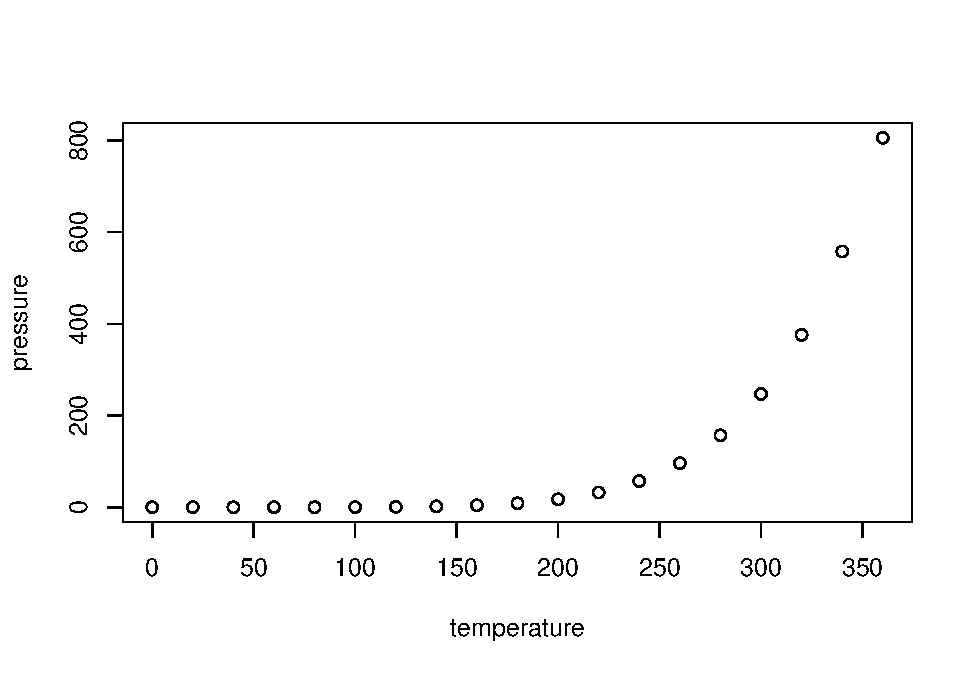
\includegraphics{est46114_s01_algebramatricial_svm_files/figure-latex/pressure-1.pdf}

\subsection{ggplot code}\label{ggplot-code}

\begin{Shaded}
\begin{Highlighting}[]
\NormalTok{df <-}\StringTok{ }\KeywordTok{data.frame}\NormalTok{(}\DataTypeTok{x =} \KeywordTok{rnorm}\NormalTok{(}\DecValTok{1000}\NormalTok{))}
\NormalTok{x <-}\StringTok{ }\NormalTok{df}\OperatorTok{$}\NormalTok{x}
\NormalTok{base <-}\StringTok{ }\KeywordTok{ggplot}\NormalTok{(df, }\KeywordTok{aes}\NormalTok{(x)) }\OperatorTok{+}\StringTok{ }\KeywordTok{geom_density}\NormalTok{()  }\OperatorTok{+}\StringTok{ }\KeywordTok{scale_x_continuous}\NormalTok{(}\DataTypeTok{limits =} \KeywordTok{c}\NormalTok{(}\OperatorTok{-}\DecValTok{5}\NormalTok{, }\DecValTok{5}\NormalTok{))}
\NormalTok{base }\OperatorTok{+}\StringTok{ }\KeywordTok{stat_function}\NormalTok{(}\DataTypeTok{fun =}\NormalTok{ dnorm, }\DataTypeTok{colour =} \StringTok{"red"}\NormalTok{)}
\end{Highlighting}
\end{Shaded}

\subsection{Another Plot}\label{another-plot}

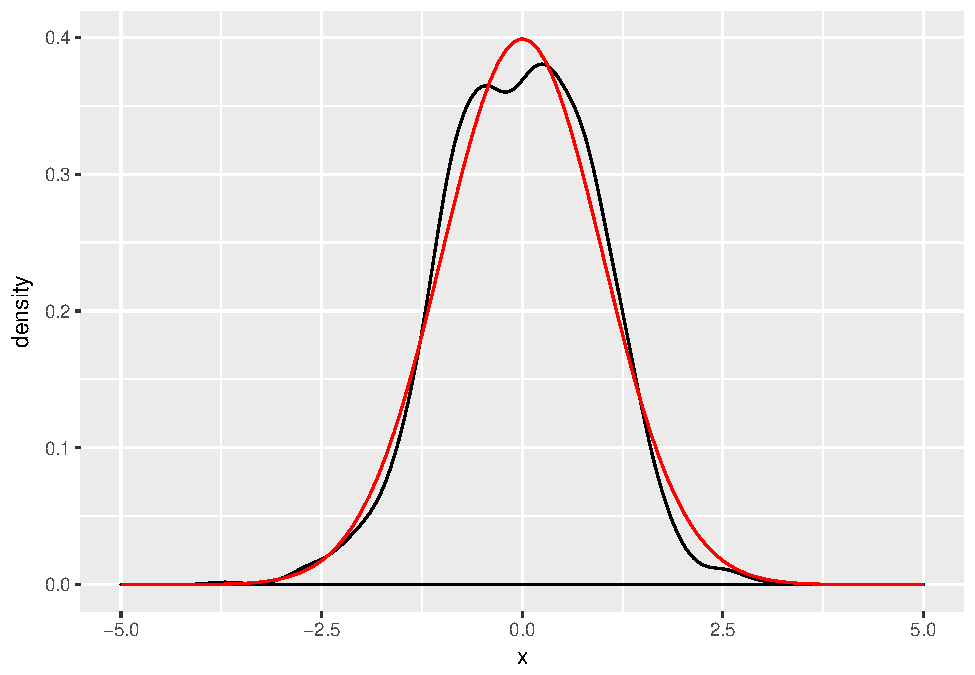
\includegraphics{est46114_s01_algebramatricial_svm_files/figure-latex/plotit-1.pdf}




\newpage
\singlespacing 
\end{document}
